\section{Kryptologische Anwendungen und Protokolle – Teil 2}

\subsection{Altersvergleich}
Führen Sie das Protokoll zum Altersvergleich mit folgenden Parametern durch.
$ 0 \le a, b \le 4$, der öffentliche RSA-Schlüssel von Bob lautet $n=143, e=19, x = 102$.
Als Einwegfunktion verwenden Sie eine Reduktion $\mod 53$.
Geben Sie die notwendigen Berechnungen, die ausgetauschten Nachrichten und das
Ergebnis für folgende Alter von Alice und Bob an:

\begin{align}
	p &= 11 & q &= 13 &	d &= 19
\end{align}

\subsubsection{$a=1, b=1$}

\begin{tabular}{lcl}
	Alice 	&& Bob                       \\
	$x=102$                             \\
	$c = E_{PK-B}(x)=102^{19} \mod 143$ \\
	$d = c-a = 15 - 1$     & \rarr &       \\
    &  &   $y = D_{SK-B}(14+0,14+1,14+2,14+3,14+4)$ \\
    &  &   $~ = (92, 102, 42, 134, 8) $             \\
    &  &   $z = (39, 49, 42, 28, 8)$	  \\
    &\larr & $(39, 49, 42+1, 28+1, 8+1)$\\
	$f(x)=49 \in z$ &  & 
\end{tabular}

\subsubsection{a=1, b=3}

\begin{tabular}{lcl}
	Alice 	&& Bob                       \\
    &\larr & $(39, 49, 42, 28, 8+1)$\\
	$f(x)=49 \in z$ &  & 
\end{tabular}

\subsubsection{a=1, b=0}

\begin{tabular}{lcl}
	Alice 	&& Bob                       \\
    &\larr & $(39, 49+1, 42+1, 28+1, 8+1)$\\
	$f(x)=49 \notin z$ &  & 
\end{tabular}

Angenommen Bob verzichtet leichtsinnigerweise auf die Anwendung der
Einwegfunktion. Zeigen Sie im Fall b) wie Alice Bobs Alter rekonstruieren kann.

\begin{align}
	z &= 	D_{SK-B}(14+2+1,14+3+1,14+4+1,14+0,14+1) \\
	  &=    E_{PK-B}(D{SK-B}(14+2+1,14+3+1,14+4+1,14+0,14+1)) \\
	  &=    (14+2+1,14+3+1,14+4+1,14+0,14+1) \\ 
	  &=    (2+1, 3+1,4+1, 0, 1) \\
\text{sort}	  &=    (0,1,3,4,5)          
\end{align}

Wert $2$ fehlt, daher $b=2$.


\subsection{No-Key-Protokoll}
Führen Sie das No-Key-Protokoll mit folgenden Parametern durch:
\[ p = 17, a = 3, b = 5 , s = 2 \]
Skizzieren Sie den Protokollablauf, berechnen Sie die ausgetauschten Werte und
rekonstruieren Sie das Geheimnis.

\begin{align}
	a' & = 11  & b' &= 13
\end{align} 

\begin{align}
	s' &= s^{ab} \mod p \\
	   &= 2^{3\cdot 5} \mod 17\\
	   &= 9
\end{align}

\begin{align}
     s &= s'^{b'a'} \mod p \\
	   &= 9^{13\cdot 11} \mod 17\\
	   &= 2
\end{align}


\subsection{(4,6)-Schwellwertverfahren über Gleichungssystem}
Es seien $p=19$ und die folgenden Wertepaare gegeben: $(1,7), (2,3), (3,4), (16, 4),
(17,5)$ und $(18,1)$. Rekonstruieren Sie aus $(1,7), (2,3), (17,5)$ und $(18,1)$ das
Geheimnis und das Polynom durch Lösen des entsprechenden linearen
Gleichungssystems.
Zeichnen Sie das Polynom für die Wert von $x=0$ bis $x=20$.

4 Freiheitsgrade = Polynomd 3. Grades: $a_3 x^3 +a_2 x^2 +a_1 x^1 +a_0 = y$.
Gesucht Koeffizienten $a_i$:

\begin{align}
	\begin{pmatrix}
1 & 1 & 1 & 1 \\ 
8 & 4 & 2 & 1 \\ 
4913 & 289 & 17 & 1 \\ 
5832 & 324 & 18 & 1
\end{pmatrix} 
\cdot  \begin{pmatrix} a_3 \\ a_2 \\ a_1 \\ a_0  \end{pmatrix} 
=  \begin{pmatrix} 7 \\ 3 \\ 5 \\ 1  \end{pmatrix} 
\end{align}

\begin{align} a = 
\begin{pmatrix}
15 \\ 6  \\ 6 \\ 18 \\
\end{pmatrix} \imp 15 x^3 + 6 x^2 +6 x^1 +18
\end{align}

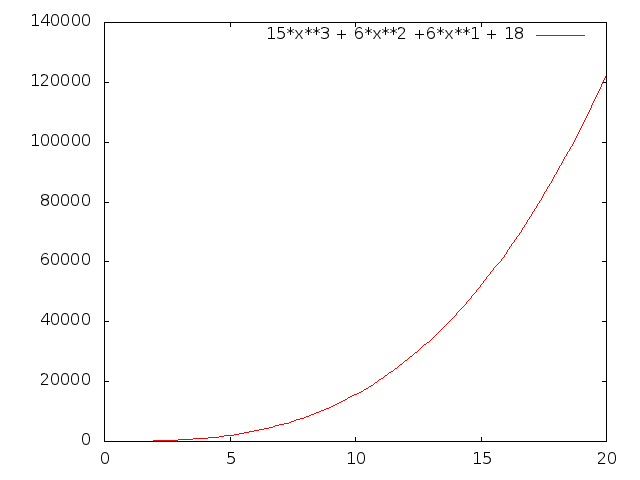
\includegraphics[scale=0.5]{images/ueb82_3.png}

\subsection{(3,4)-Schwellwertverfahren über Lagrange}
Gegeben sind folgende Punkte (1,6) (2,3), (3,2), (4,3).
Wählen Sie drei Punkte aus und rekonstruieren Sie das Polynom über das
Lagrangesche-Interpolationspolynom.
Was ist das Geheimnis? Zeichen Sie das Polynom.
